\documentclass{article}
\usepackage{graphicx}
\usepackage{amsmath, amsfonts, mathtools}
\usepackage{amsthm}
\usepackage{todonotes}
\usepackage[ruled, linesnumbered]{algorithm2e}
\usepackage{enumerate}
\usepackage{float}
\usepackage{subcaption}
\usepackage{dsfont}
\usepackage{pythonhighlight}
\usepackage{listings}
\usepackage{xcolor}
\usepackage{xurl}
\usepackage{algorithm2e}

% Define colors for syntax highlighting
\definecolor{codegreen}{rgb}{0.2,0.6,0.2}
\definecolor{codegray}{rgb}{0.5,0.5,0.5}
\definecolor{codepurple}{rgb}{0.58,0,0.82}
\definecolor{backcolour}{rgb}{0.95,0.95,0.92}


% Sensible defaults for lstlistings
\lstset{
numberstyle=\tiny\color{codegray},
backgroundcolor=\color{backcolour},   
  basicstyle=\footnotesize\ttfamily,
  belowcaptionskip=1\baselineskip,
  breaklines=true,
  commentstyle=\bfseries\color{purple!40!black}
  frame=L,
  identifierstyle=\color{blue},
  keywordstyle=\bfseries\color{green!40!black},
  language=python,
  showstringspaces=false,
  stringstyle=\color{orange},
  xleftmargin=\parindent,
  captionpos=b,                    
    keepspaces=true,                 
    numbers=left,                    
    numbersep=5pt,                  
    showspaces=false,                
    showstringspaces=false,
    showtabs=false,
    tabsize=2,
    framexleftmargin=16pt,
    framextopmargin=6pt,
        framexbottommargin=6pt, 
        frame=tb, framerule=0pt,
}


\title{Approximation Algorithms - Assignment 3}
\author{Group 2: Christoph Kern, Johannes Gabriel Sindlinger}


\begin{document}

\maketitle

\section{Scheduling Jobs with Precedence Constraints}
\fbox{\begin{minipage}{0.98\textwidth}
    We consider scheduling jobs on identical machines as in Section 2.3, but jobs are now subject to \emph{precedence constraints}. We say $i \prec j$ if in any feasible schedule, job $i$ must be completely processed before job $j$ begins processing. A natural variant on the list scheduling algorithm is one in which whenever a machine becomes idle, then any remaining job that is available is assigned to start processing on that machine. A job $j$ is available if all jobs $i$ such that $i \prec j$ have already been completely processed. Show that this list scheduling algorithm is a $2$-approximation algorithm for the problem with precedence constraints.
\end{minipage}}

\begin{proof}
    First, let us model the precedence relations between the jobs as a directed graph $G=(V,E)$, where
    \begin{align*}
        V &= \{1,\dots,n\}\\
        E &= \{(i,j)\ |\ \forall i,j \in V,\ i \prec j\}
    \end{align*}
    Let $P$ be some path of $G$. Due to the transitive properties of the precedence relation, any job $i$ of $P$ that is followed by some job $j$ in $P$ must also be completely processed before job $j$ is executed in our schedule. Thus, any two jobs in $P$ can not run simultaneously. Note that $G$ must form a directed acyclic graph (DAG) as otherwise we would have cyclic dependencies between the jobs, making it impossible to schedule them. Let $A$ be some subset of jobs of some path $P$ in $G$. Since all jobs in $A$ can at best be executed one after another, we can establish following lower bound on the length of an optimal schedule $C^*_{\max}$:
    \[
        C^*_{\max} \ge \sum_{i \in A} p_{i}
    \]
    Like in the original problem, we also have following lower bound:
    \[
        C^*_{\max} \ge \frac{\sum^n_{j=1}p_j}{m}
    \]

    Now consider a solution of the modified list scheduling algorithm in which some job $j_1$ completes last in the final schedule. The completion time of job $j_1$, $C_{j_1}$, is equal to this solution's objective function value. Before the start of job $j_1$, $S_{j_1}$, either all machines are busy or there are timeslots in which at least one machine is idle. In the latter case, consider the end time of such a timeslot closest to $S_j$, denoted by $t_j$. Then there must be some job $j_2$ preceded by job $j_1$ in $G$ that is executing at time $t_1$ (i.e.~there is a path from $j_2$ to $j_1$ in $G$). This must be the case as otherwise the list scheduling algorithm could have executed $j_1$ or some predecessor of $j_1$ before $t_1$ on the idle machine. We now repeat this procedure for job $j_2$ in an inductive fashion, resulting in a set of jobs $A$. Below, you will find pseudo-code describing the same procedure:

    \begin{algorithm}
        \caption{Construction of $A$}
        \label{alg:1}
        \KwIn{Job $j_1$ that completes last in the final schedule}
        \KwOut{Set of jobs $A$}
        $A \coloneqq \{j_1\}$\\
        $j \coloneqq j_1$\\
        \While{there is a timeslot where a machine is idle in $[0, S_j]$}{
            $t \coloneqq$ end time of closest such timeslot to $S_j$\\
            $j' \coloneqq$ job that is executed at $t$ which precedes $j$ in $G$\\
            $A \coloneqq \{j'\}$\\
            $j \coloneqq j'$
        }
        \Return{$A$}
    \end{algorithm}

    Following properties of $A$ are a consequence of this construction:
    \begin{enumerate}
        \item The jobs of $A$ are a subset of some path in $G$
        \item In $[0, C_{j_1}]$, in all timeslots in which none of the jobs of $A$ are running, all machines are busy.
    \end{enumerate}
    Thus, $C_{j_1}$ is equal to the cumulative processing time of $A$ plus the timeslots in-between in which all machines are busy. As the latter can be at most $\frac{\sum^n_{j=1}p_j}{m}$, we establish following upper bound on $C_{j_1}$:
    \[
        C_{j_1} \le \sum_{j \in A} p_j + \frac{\sum^n_{j=1}p_j}{m}
    \]
    By applying the previously defined lower bounds on $C^*_{\max}$, we can show that the modified scheduling algorithm is a 2-approximation:
    \[
        C_{j_1} \le \sum_{j \in A} p_j + \frac{\sum^n_{j=1}p_j}{m} \le C_{\max}^* + C_{\max}^* = 2 \cdot C_{\max}^*
    \]
\end{proof}




\section{Asymmetric TSP}

\fbox{\begin{minipage}{0.98\textwidth}
    The Wikipedia article on TSP claims that it is possible to solve TSP in the setting where distances are asymmetric, by reducing this to the standard (symmetric) case. In the reduction some vertices that have "no edges" between them; you can think of this as having infinite (or very large) weight. Explain how to choose the value $w$ and argue that the reduction is correct.  Why does this reduction not imply a $\frac{3}{2}$-approximation for the asymmetric TSP?
\end{minipage}}

\begin{proof}
    We aim to show that the reduction is correct. Let $G=(V,E)$ be the original complete graph ($|V| = n$). The reduced graph $G'=(V',E')$ is a complete graph where we mirror each vertex in $V$, i.e.
    \[
        V' = \{v_i, v_i'\ |\ v_i \in V\}
    \]
    We refer to the mirrored vertices as ghost vertices (indicate by $'$). The vertices between an original vertex $v_i \in V'$ and its corresponding ghost vertex $v_i' \in V'$ will be referred to as a ghost edges. 

    The asymmetric weights $w_{v_i \to v_j}$ of $G$ will be mapped to symmetric weights in our constructed graph as follows:
    \[
        w_e = \begin{cases}
            w_{v_i \to v_j} & \text{if }e = \{v_i', v_j\}\\
            w & \text{if }e = \{v_i, v_i'\}\\
            \infty & \text{otherwise}
        \end{cases} \text{ for every } e \in E'
    \]

    The weight $w$ of the ghost edges will be defined later in the reduction. Edges between two original vertices or between two ghost vertices will have infinite weight, as they are not supposed to be used.
    
    
    We claim that there exists a tour $C$ in $G$ such that $\text{cost}(C) \le d$ iff there exists a tour $C'$ in $G'$ such that $\text{cost}(C') \le d + n \cdot w$. We show the correctness of both directions of this equivalence relation.

    \begin{itemize}
        \item[$(\Rightarrow)$]  Let $C = v_1 \rightarrow v_2 \rightarrow \dots \rightarrow v_n \rightarrow v_1$ be a tour of $G$ such that $\text{cost}(C) \le d$. We can create an equivalent tour $C' = v_1 \rightarrow v_1' \rightarrow v_2\rightarrow v_2' \rightarrow \dots \rightarrow v_n \rightarrow v_n' \rightarrow v_1$ in $G'$, where every vertex $v_i \in V$ is simply replaced by the sequence $v_i \rightarrow v_i'$. Since every vertex must be part of the tour, also all ghost edges must be part of our constructed tour, which together adds a cost of $n \cdot w$. Since the remaining edges are equivalent to those of the original tour, also in terms of weight, we end up with \[cost(C') = cost(C) + n \cdot w \le d + n \cdot w.\]

        \item [$(\Leftarrow)$] Let $C'$ be some tour of $G'$ such that $\text{cost}(C') \le d + n \cdot w$. If $C'$ contains two consecutive original vertices or two consecutive ghost vertices, then $cost(C') = \infty$. As $w$ is finite, we have $d = \infty$. As any tour in $G$ will have a cost less than or equal to $\infty$, it will also have a cost less than $d$. 
        
        Now consider the case where we only have alternating original and ghost vertices. Furthermore, lets restrict ourselves to the case where all ghost edges are traversed by the tour. W.l.o.g.~suppose the tour starts at the original vertex $v_1$ and is followed by ghost vertex $v_1'$ (otherwise traverse the tour in the other direction; this must be equivalent in cost due to symmetry). Then the tour $C'$ must have following shape:
        \[
            C' = v_1 \rightarrow v_1' \rightarrow v_2'\rightarrow v_2' \rightarrow \dots \rightarrow v_n \rightarrow v_n' \rightarrow v_1
        \]
        
        We can then merge all regular vertices with its corresponding ghost vertex in the tour which results in a tour $C$ for $G$, where the edges have the same weight as the edges in $C'$ without the ghost edges. Since $\text{cost}(C) = \text{cost}(C') - n \cdot w$, we have $\text{cost}(C) \le d$.

        Finally, suppose the tour $C'$ does not contain the ghost edge $\{v_i, v_i'\}$. We will now show how to construct a tour $C''$ of $G$ from $C'$ which contains the ghost edge $\{v_i, v_i'\}$ such that $\text{cost}(C'') \le \text{cost}(C')$. This procedure can then be applied for every ghost edge, which allows us to use the above construction for a tour $C$ in $G$, resulting in $\text{cost}(C) \le d$.

        \begin{figure}
            \centering
            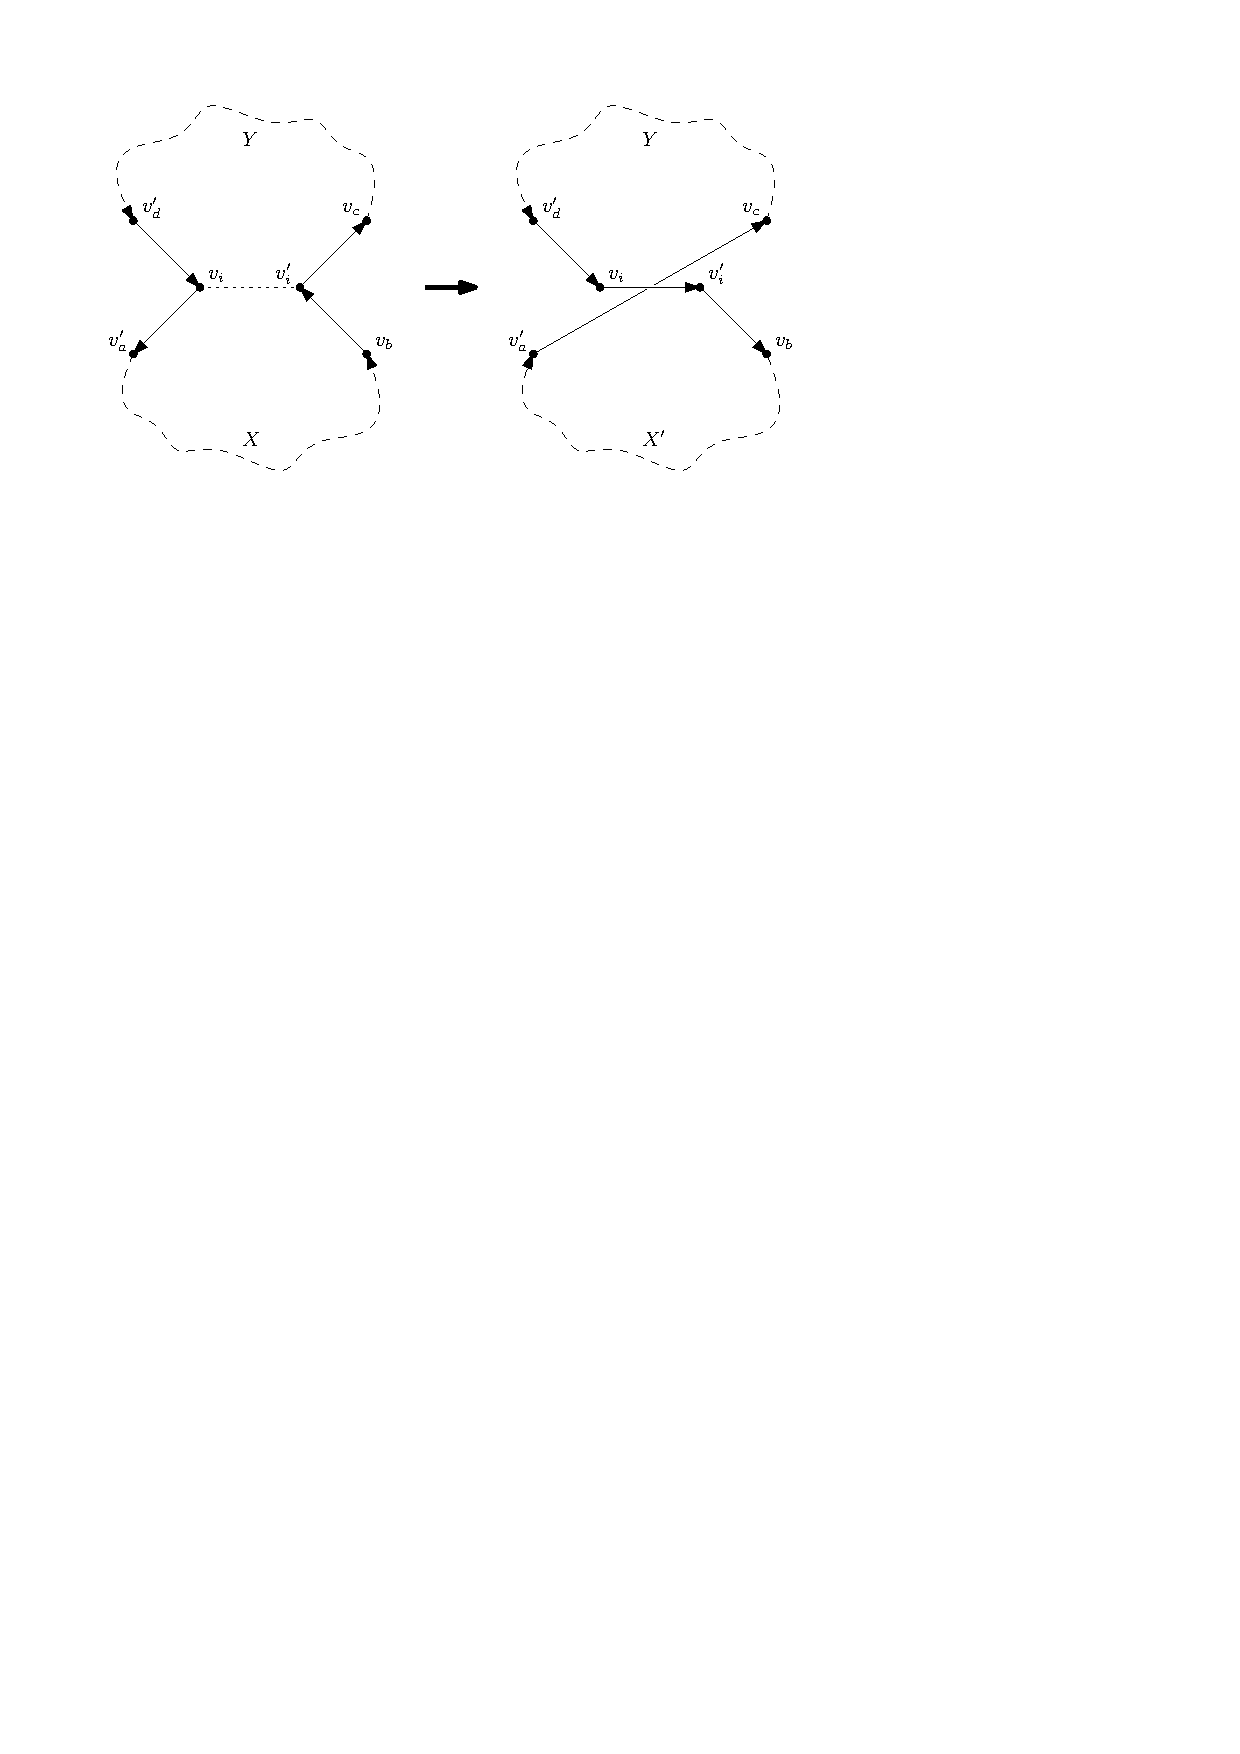
\includegraphics{Assignment3/figures.pdf}
            \caption{Process of adding ghost edge to tour}
            \label{fig:no_ghost}
        \end{figure}

        W.l.o.g.~let $C'$ start with vertex $v_i$, such that
        \[
            C' = v_i \to X \to v_i' \to Y \to v_i
        \]
        where $X$ and $Y$ are two vertex disjoint paths. Since the vertices alternate between original and ghost vertex, it must be that $X$ starts with some ghost vertex $v_a'$ and ends with some original vertex $v_b$, whereas $Y$ must start with some original vertex $v_c$ and end with some ghost vertex $v_d'$. Let $X'$ be the path obtained from reversing $X$, then we construct $C''$ as follows:
         \[
            C'' = v_i \to v_i' \to X' \to Y \to v_i
        \]
        Figure~\ref{fig:no_ghost} demonstrates this visually. Notice that the resulting tour still has alternating original and ghost vertices. Observe that we remove edges $\{v_i, v_a'\}$ and $\{v_i', v_c\}$, but add the ghost edge $\{v_i, v_i'\}$ and edge $\{v_a', v_c\}$. Thus, $cost(C'') \le cost(C')$ iff $w_{a \to c} + w \le w_{a \to i} + w_{i \to c}$. Consequently, $w \le w_{a \to i} + w_{i \to c} - w_{a \to c}$ must hold. Note that if the triangle inequality holds, i.e.~$w_{a \to c} \le w_{a \to i} + w_{i \to c}$, then $w=0$ would suffice. Otherwise, we need to consider every set of 3 vertices in $V$, and use this to bound $w$.
    \end{itemize}
    Now that we have shown the correctness of the reduction, we want to argue why this does not imply a $\frac{3}{2}$-approximation for the asymmetric TSP. We observe that the constructed graph $G'$ is not metric as the triangle inequality does not hold. Consider a set of three vertices of $G'$ consisting of two original vertices $v_i, v_j$ and one ghost vertex $v_k'$. Then $w_{\{v_i, v_j\}} \le w_{\{v_i, v_k'\}} + w_{\{v_k', v_j\}}$ may not hold, since $w_{\{v_i, v_j\}}$ is infinite and $w_{\{v_i, v_k'\}}$ and $w_{\{v_k', v_j\}}$ are usually finite. Since the demonstrated approximation scheme needs the TSP problem to be metric, this does not imply a $\frac{3}{2}$-approximation.
\end{proof}
\end{document}
